
\begin{figure}
    \centering
    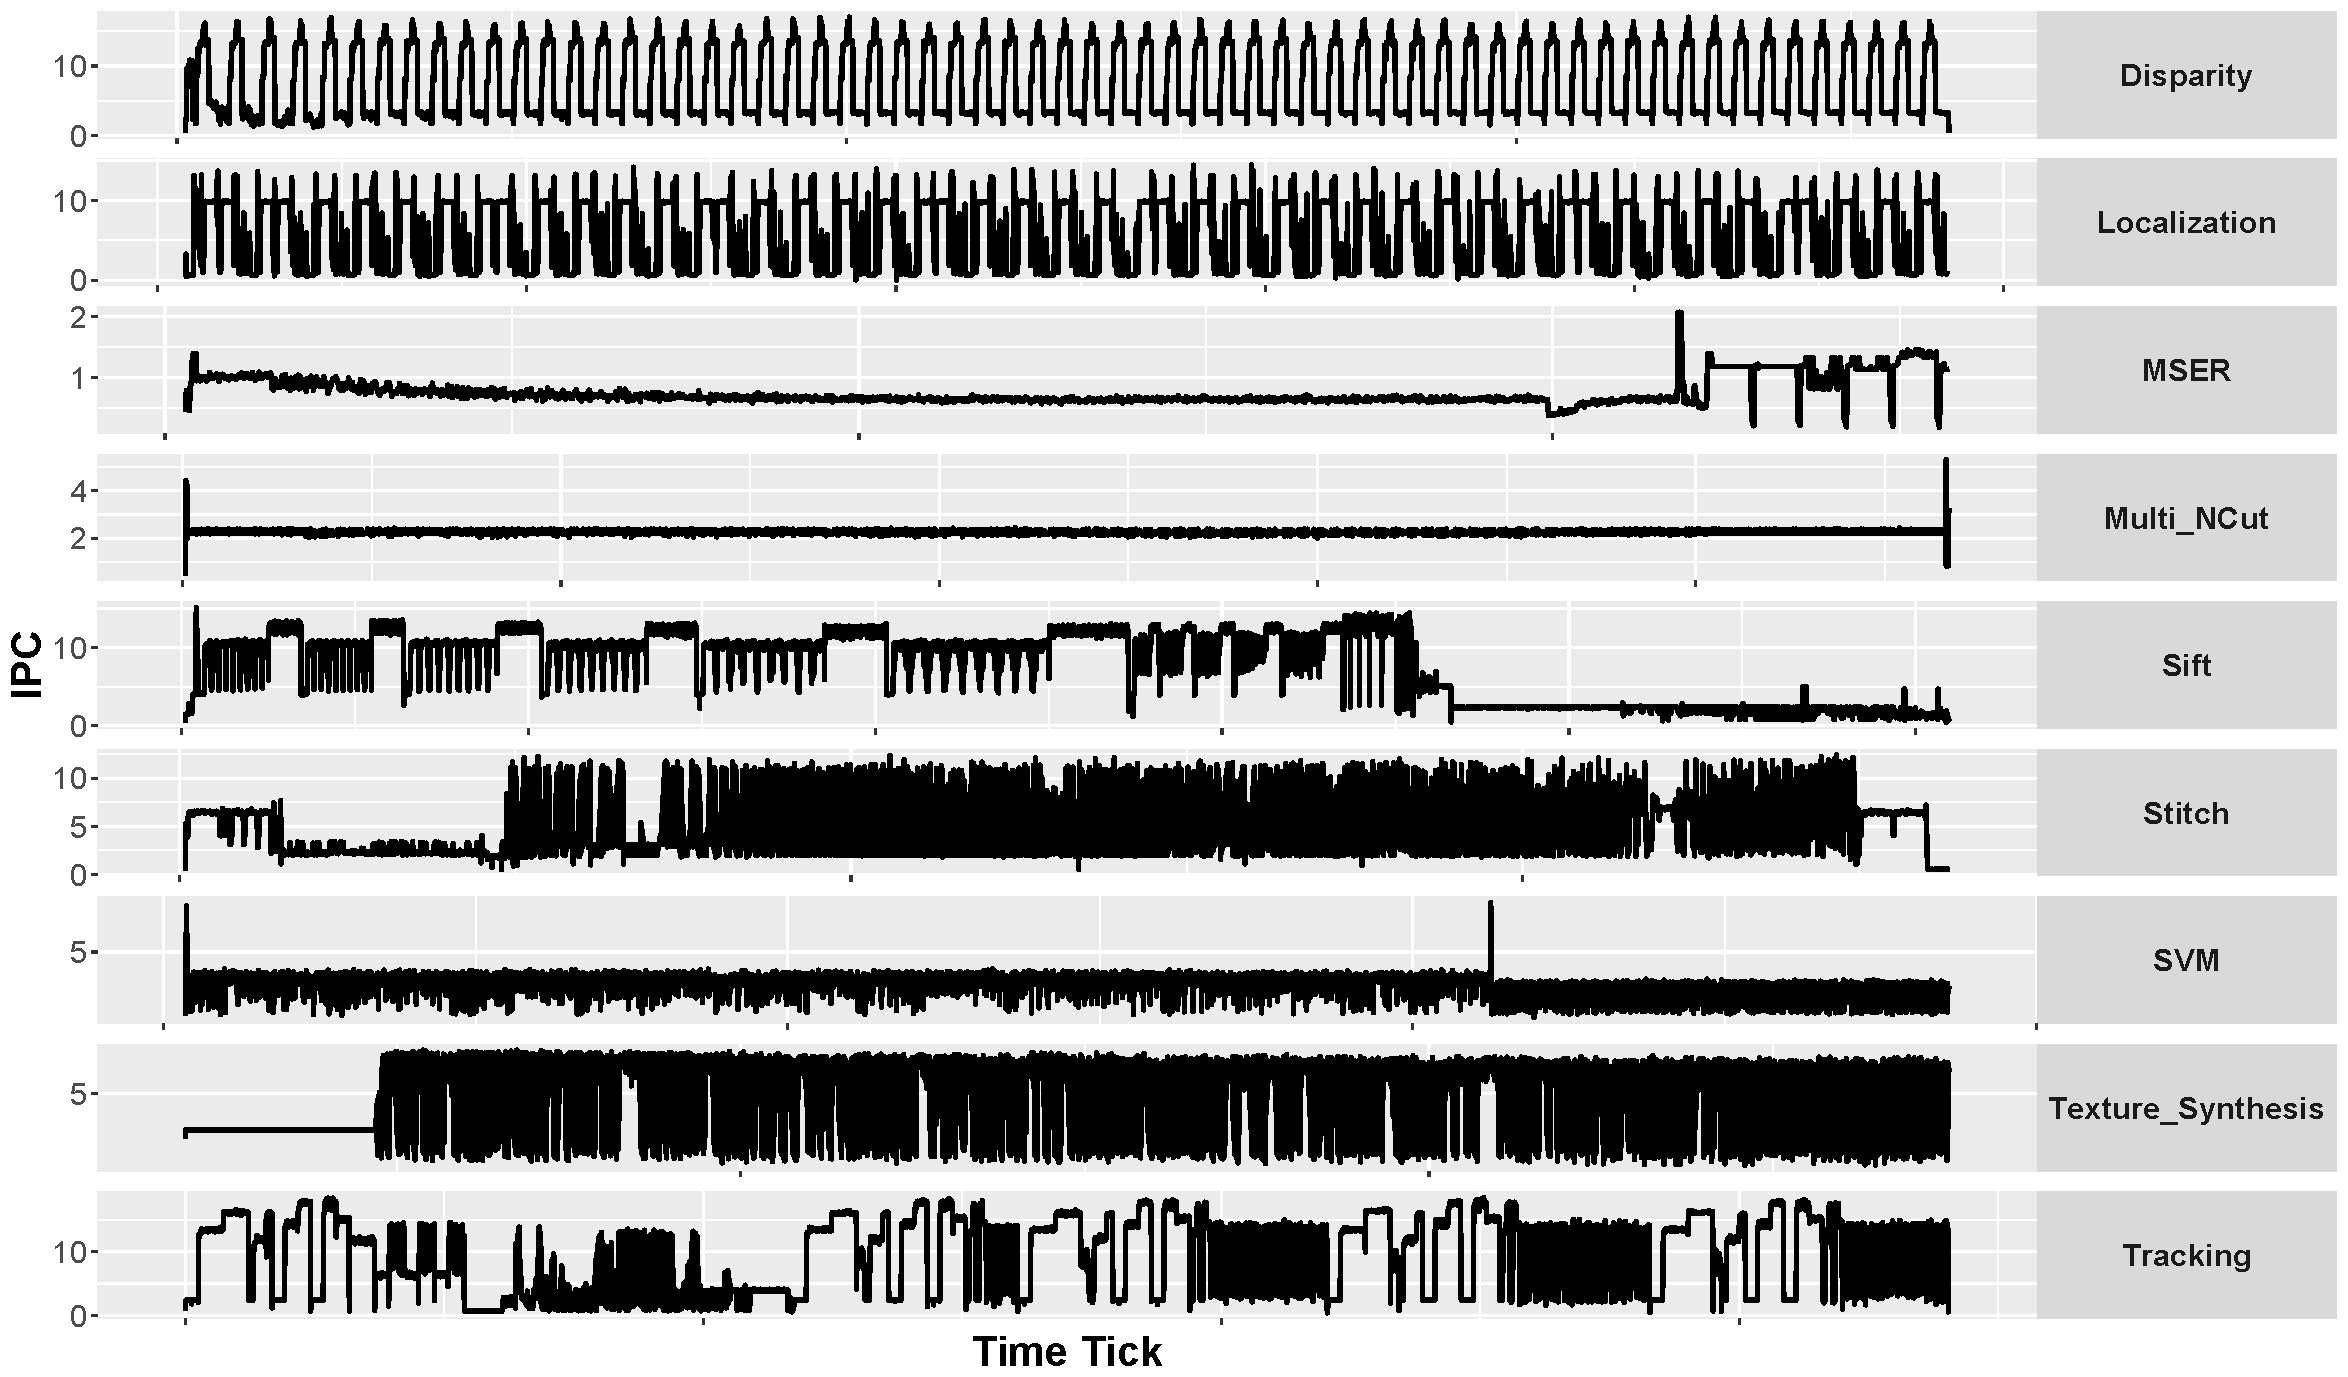
\includegraphics[width=1\textwidth]{cases-paper/graphics/Exploration/ipcs_16_2.pdf}
    \caption{IPC as a function of time for each benchmark when run on 16 fused cores.}
    \label{fig:sxt}
	\vspace{1em}
\end{figure}

This section explores how core composition affects the performance of the SD-VBS benchmarks.
First a phase analysis is performed, followed by a study of the IPC variation for static core fusion.
Then the use of dynamic core composition is motivated by using the gathered information.


\begin{figure}[t]
    \centering
    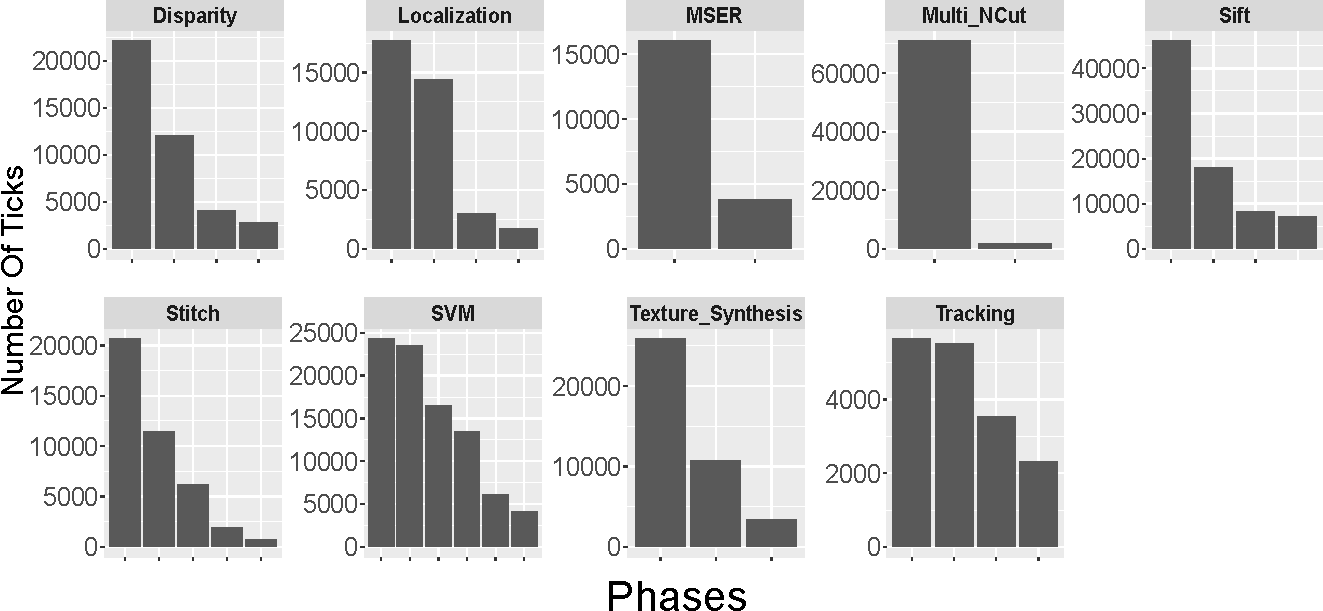
\includegraphics[width=1\textwidth]{cases-paper/graphics/Exploration/clusters3.pdf}
    \caption{Number of phases determined for each benchmark using kMeans clustering and their distribution.}
    \label{fig:clust}
		\vspace{5mm}
\end{figure}


\subsection{Phase Detection}
Figure~\ref{fig:sxt} presents the IPC performance through time for all the benchmarks when using a logical core (LC) composed of 16 cores.
The IPC is calculated for each time tick, which is set at interval of 640 blocks committed.
The IPC varies a lot for some of the benchmarks such as \bm{Disparity} or \bm{Localization} where dynamic fusion is expected to be especially good.
For other, such as \bm{Multi\_NCut}, the execution is dominated by a single long phase with constant IPC, which will clearly show no benefit from using dynamic fusion.

To better understand how dynamic core fusion improves performance, either by improving speedup or reducing energy, this section begins with a study of how each benchmark features different phases during their execution.
For every benchmark the IPC results of 16,8,4,2,1 fused cores are regrouped and kMeans clustering is applied to determine phases.
This process is only done for the purpose of exploring this set of benchmarks.
Intervals that exhibit similar IPC values when run on different core counts are classified in the same cluster.
In order to find the correct number of clusters the Sum of Square Errors (SSE) is plotted for a given cluster size from 1 to 15 and determine the optimal cluster to be in the elbow in the plot~\cite{everitCluster2001}.

Figure~\ref{fig:clust} shows us the optimal number of clusters for each benchmark and the frequency of each cluster.
The data can be corroborated with the information found in Figure~\ref{fig:sxt}.
For example, benchmarks \bm{MSER} and \bm{Multi\_NCut} feature two phases, with one dominating phase.
This means that it will be impossible to obtain any kind of performance improvements through dynamic reconfiguration.
For all the other benchmarks, they each have at least two dominant phases.
Since each phase is a cluster of similar IPC values, having two or more clusters will result in a higher chance of benefiting from dynamic core fusion.


\begin{figure}
    \centering
    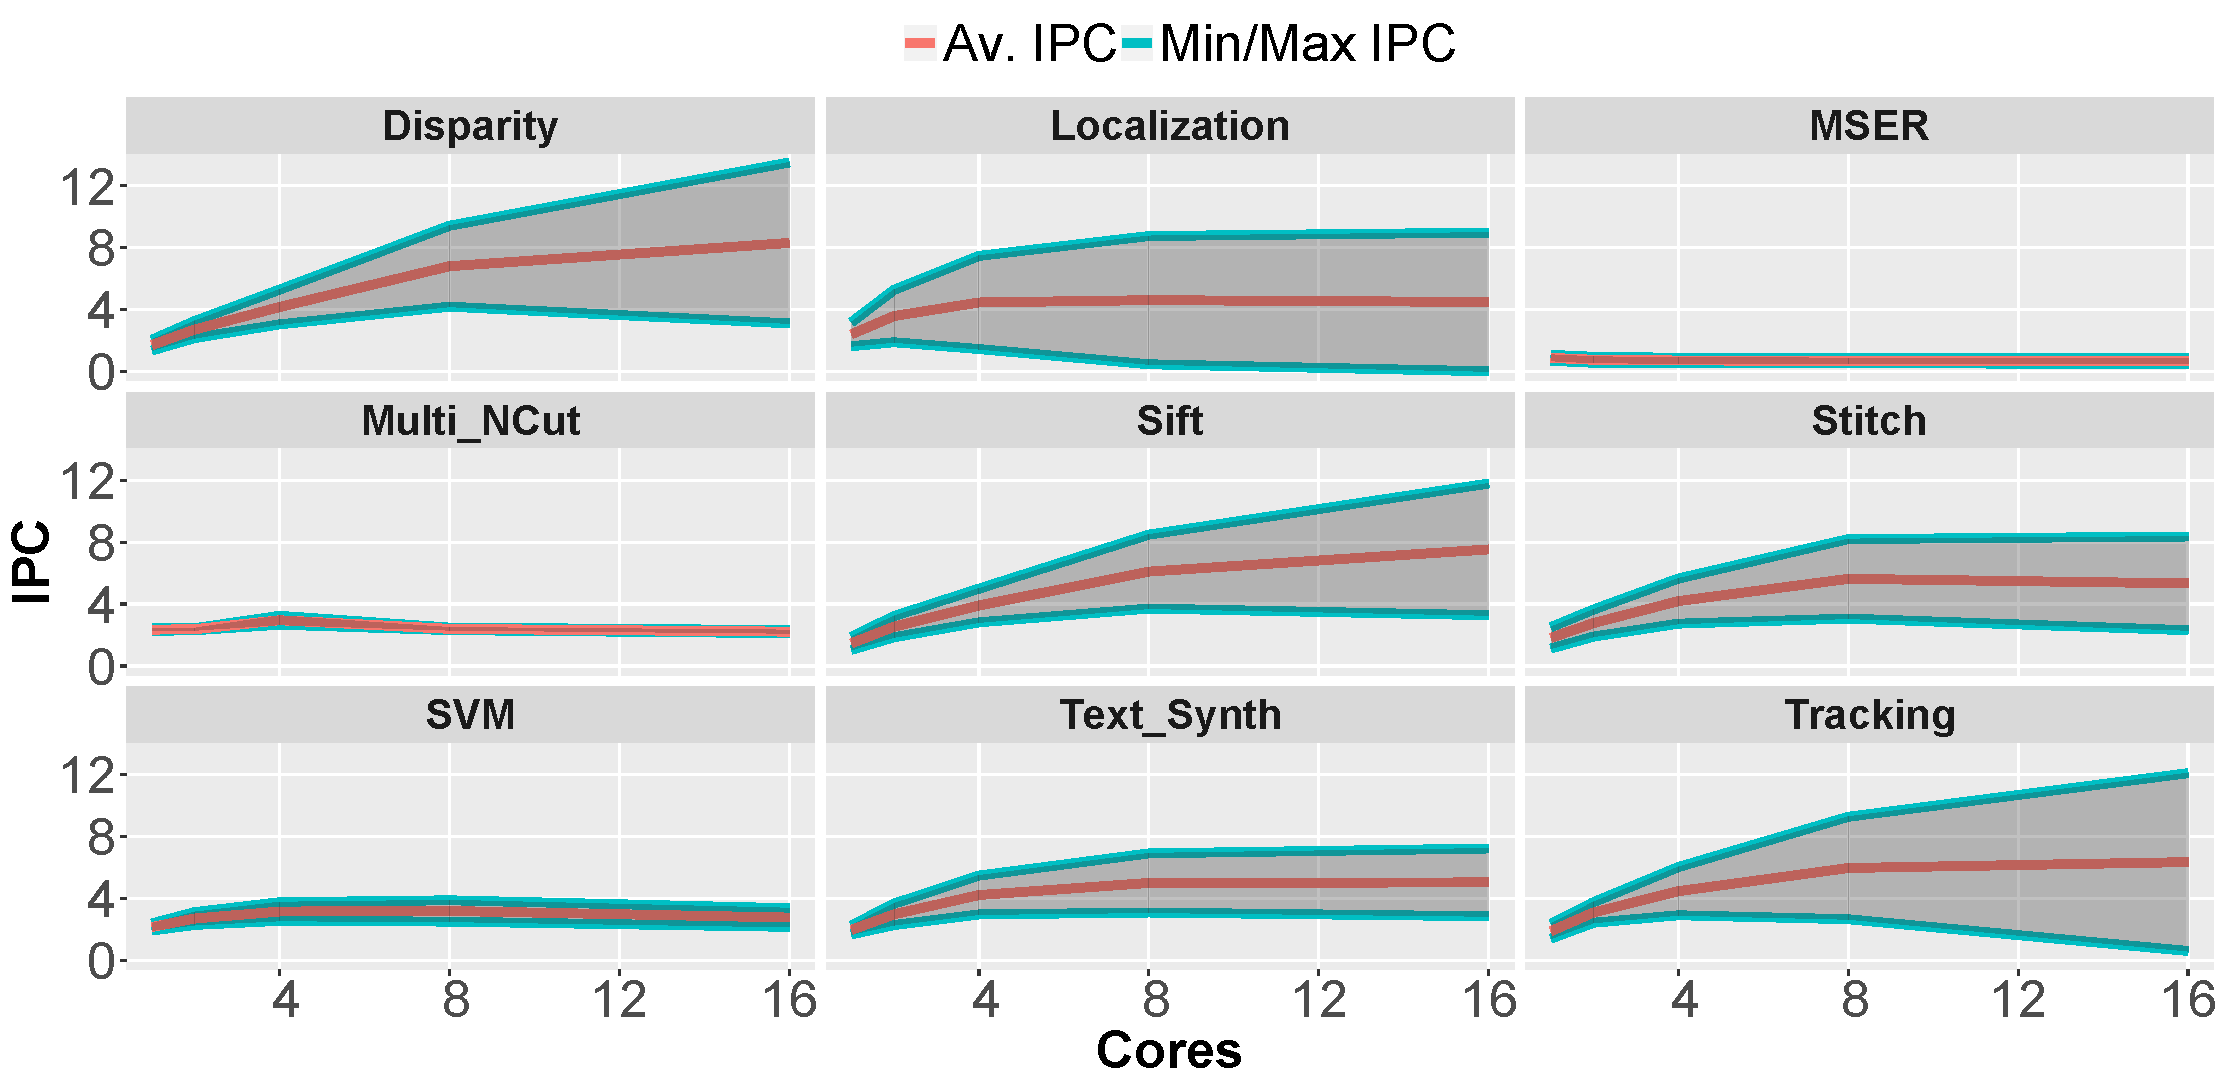
\includegraphics[width=1\textwidth]{cases-paper/graphics/Exploration/stddev2.pdf}
    \caption{Comparing average, smallest and greatest IPC for each SD-VBS benchmark using logical-core size of 16.}
    \label{fig:stddev}
		\vspace{5mm}
\end{figure}

\begin{figure}[t]
    \centering
    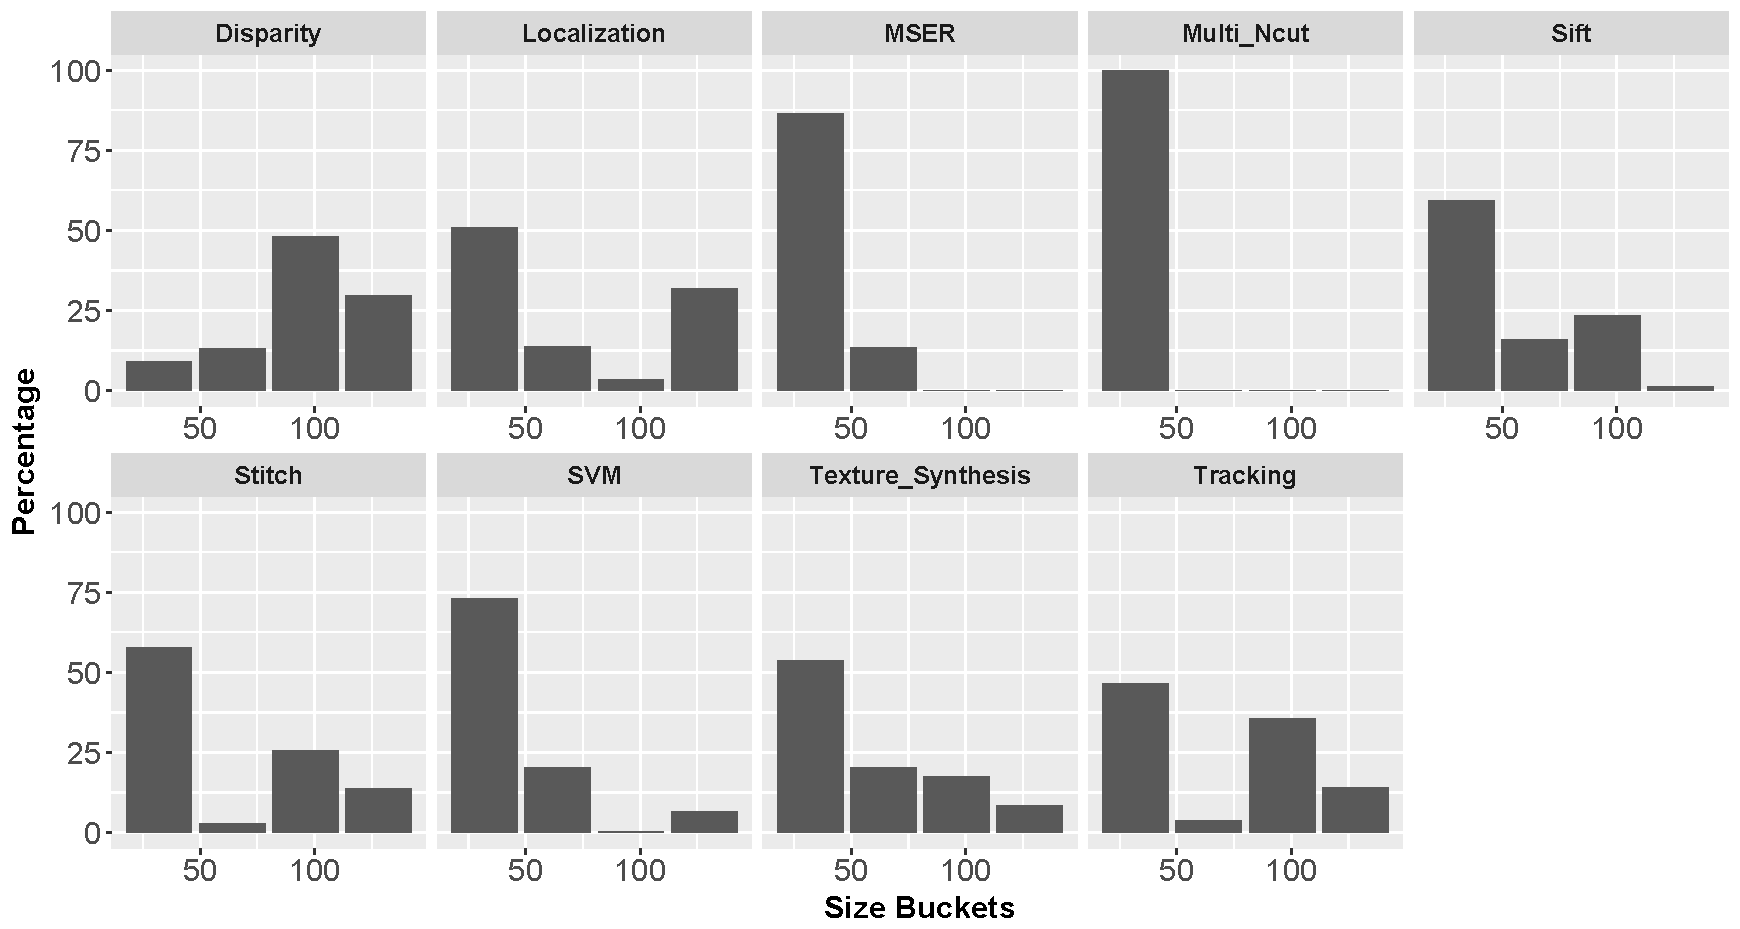
\includegraphics[width=1\textwidth]{cases-paper/graphics/Exploration/SizeBuckets.pdf}
    \caption{Distribution of block sizes for each benchmark. The sizes are clustered in buckets equivalent to number of lanes occupied.}
    \label{fig:block_sizes}
	\vspace{5mm}
\end{figure}
\subsection{Static Core Fusion Exploration}

Figure~\ref{fig:stddev} shows how the average Instructions Per Cycle (IPC) changes as the size of a LC is increased, going in powers of 2 from 1 to 16 fused cores.
It can be seen that, for most benchmarks, fusing more cores provides an increase in IPC performance.
Benchmarks \bm{Disparity}, \bm{Localization}, \bm{Sift}, \bm{Stitch}, \bm{Texture Synthesis} and \bm{Tracking} all at least observe a speedup of 2x when using core fusion.

However increasing the size of a LC is not always beneficial as can be seen in benchmarks \bm{Localization}, \bm{MSER}, \bm{Multi\_NCut}, \bm{Stich}, and \bm{SVM}.
For benchmarks \bm{Localization} and \bm{Stitch} the performance increases when fusing up to 8 cores, where-as \bm{MSER} and \bm{Multi\_NCut} never benefit from core fusion. 
Referring back to Figures~\ref{fig:sxt} and~\ref{fig:clust}, \bm{MSER} and \bm{Multi\_NCut} feature one dominating long phase, both performing poorly.
Figure~\ref{fig:block_sizes} shows the distribution of block-sizes for each of the benchmarks.
As fine-grained sizes do not matter as much as overall number of lanes being occupied, the block sizes are clustered into groups which represent how ever many number of lanes will be occupied (one lane may execute a block of up to 32 instructions).

Figure~\ref{fig:block_sizes} helps explain why benchmarks \bm{MSER} and \bm{Multi\_NCut} do not perform any better with core-fusion.
For both cases, not only do they have a single detected phase, but both are predominantly formed of blocks that will occupy a single lane.
In fact, the most frequent block in \bm{MSER}, comprising 21\% the total executed blocks are comprised of only 8 instructions, whilst 31\% of \bm{Multi\_NCut}'s blocks are of 28 instructions.
Having such small blocks will always increase both the \textit{SynchronizationCost} and the branch-prediction requirements.
For \bm{MSER}, the fact that an important percentage of blocks are only 8 instructions long signifies that the overhead of fetching enough blocks for a large core-composition and the synchronization cost for committing them outweighs executing the blocks on a single core.
The reason there is no degredation of performance is due to the fact that when fusing a high amount of cores, if the overhead of fetching the blocks outweighs the time required to execute them, cores will simply not execute blocks.
For example, fusing 16 cores and executing \bm{MSER} may in fact result in a single core being used due to it executing blocks faster than it being able to dispatch the blocks to a next core.
Hence, in this case, \bm{MSER} would be wasting a lot of energy trying to use 16 cores in a composition, whilst effectively only executing on a single core. 
This explains the lack of scaling for these two benchmarks.

Figure~\ref{fig:stddev} also shows the standard deviation of the IPC for each given LC size represented by the grayed out areas.
For example, running the \bm{Disparity} benchmark on a LC of 16 cores, it can be observed that an average IPC of 8.3 with a standard deviation of 5.2.
The standard deviation for 16 cores shows that the performance can drop down to 2.5.
An IPC of 2.5 when using 16 cores is very inefficient as this represents 0.1 of an instruction per cycle for each core.
Using a LC of size 4 for the \bm{Disparity} benchmark an average of 4.1 with a standard deviation of 1.2 is achieved.
Thus, if the logical-core could change size, there is a possibility that this could reduce the overall energy consumption of the system by switching from 16 to 4.

Overall, most benchmarks that benefit from large logical-cores will also be met with important standard deviations of IPC performance.
The high standard deviation is evidence of performance phases found in each application which are likely to benefit from dynamic adaptation.
